\section{Introducción a la Estadística}

\mode<presentation>{
%---------------------------------------------------------------------slide----
\begin{frame}
\frametitle{Introducción a la Estadística}
\tableofcontents[sectionstyle=show/hide,hideothersubsections]
\end{frame}
}


\subsection{La estadística como herramienta científica}
%---------------------------------------------------------------------slide----
\begin{frame}
\frametitle{¿Qué es la estadística?}
\begin{definicion}[Estadística]
La \emph{estadística} es una rama de las matemáticas que se encarga de la recogida, análisis e interpretación de datos.
\end{definicion}

El papel de la Estadística es extraer información de los datos para adquirir el conocimiento necesario para tomar decisiones.

\begin{center}
\tikzsetnextfilename{introduccion/proposito_estadistica}
\resizebox{\textwidth}{!}{
% Autor: Alfredo Sánchez Alberca (email:asalber@ceu.es)
% Charts that shows the purpose of Statistics
\begin{tikzpicture}[every label/.style={text=color1}]
\tikzstyle{node} = [align=center, node distance=1cm, text=color1]; 
\tikzstyle{arrow} = [-latex, color1, line width=10pt];

\node (data) [label=-90:Datos] at (0,1) {
\includegraphics[height=1.5cm]{img/introduccion/datos.pdf}}; 
\pause
\node (information) [label=-90:Información] at (4.7,1)
{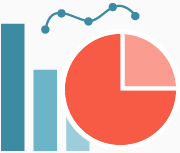
\includegraphics[height=1.5cm]{img/introduccion/informacion.png}}; 
\node at (2,1) [fill=color1,single arrow,shape border rotate=0,text=white, minimum width=1.1cm]{
\ ESTADÍSTICA\ \phantom{}};
\pause
\node (knowledge) [label=-90:Conocimiento] at (9.5,1) {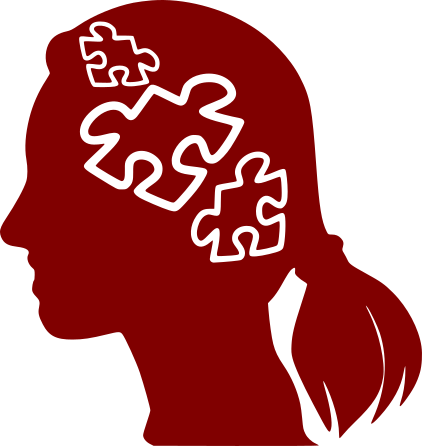
\includegraphics[height=1.5cm]{img/introduccion/conocimiento.png}};
\node at (7,1) [fill=color1,single arrow,shape border rotate=0,text=white, minimum width=1.1cm]{
Interpretación\phantom{}};
\pause
\node at (11.5,1) [fill=color1,single arrow,shape border rotate=0,text=white, minimum width=1.1cm]{
\ Decisiones\ \phantom{}};
\end{tikzpicture} 
}
\end{center}

\uncover<5->{
La estadística es imprescindible en cualquier disciplina científica o técnica donde se manejen datos, especialmente si son grandes volúmenes de datos, como por ejemplo en Física, Química, Medicina, Psicología, Economía o Ciencias Sociales.}

\uncover<6->{
\begin{center}
Pero, \alert{\emph{¿por qué es necesaria la Estadística?}}
\end{center}
}
\end{frame}


\note{La Estadística está por todas partes en el mundo que nos rodea y la usamos en multitud de ocasiones en nuestra
vida cotidiana aunque no seamos conscientes de ello. Cuando miramos una factura de la luz, o el gasto del teléfono
móvil, cuando comprobamos la popularidad de nuestros mensajes en las redes sociales, cuando vemos la posición que ocupa
nuestro equipo favorito en la clasificación de la liga, o cuando vemos las predicciones meteorológicas, estamos
usando la Estadística.
Pero formalmente, podríamos definir la Estadística como una rama de las matemáticas que se encarga de la recogida,
análisis e interpretación de datos.

Como tiene que ver con el tratamiento de datos, esto la hace imprescindible en cualquier disciplina científica o
técnica donde se manejen datos, especialmente si son grandes volúmenes de datos, como por ejemplo, la física, la
química, la medicina y las ciencias biosanitarias, pero también en la economía, la psicología o las ciencias sociales.

Pero, en realidad, ¿porqué es necesaria la estadística?
}

%---------------------------------------------------------------------slide----
\begin{frame}
\frametitle{La variabilidad de nuestro mundo}
El científico trata de estudiar el mundo que le rodea; un mundo que está lleno de variaciones que dificultan la
determinación del comportamiento de las cosas.

\begin{center}
\alert{\emph{¡La variabilidad del mundo real es el origen de la estadística!}}
\end{center}

La estadística actúa como disciplina puente entre la realidad del mundo y los modelos matemáticos que tratan de explicarla, proporcionando una metodología para evaluar las discrepancias entre la realidad y los modelos teóricos.

Esto la convierte en una herramienta indispensable en las ciencias aplicadas que requieran el análisis de datos y el diseño de experimentos.
\end{frame}
\note{Bien, podemos decir que los científicos tratamos de estudiar el mundo que nos rodea, para comprenderlo y
controlarlo. Pero vivimos en un mundo con una que está lleno de variaciones que dificultan la determinación del
comportamiento de las cosas. No hay dos personas iguales, ni dos animales iguales, ni dos plantas iguales, ni siquiera
existen dos gotas de agua iguales. Esta enorme biodiversidad, que es la mayor riqueza de nuestro mundo, es al mismo
tiempo el principal obstáculo para comprender los fenómenos naturales.

Así, cuando por ejemplo estamos estudiando una enfermedad y su cura, es posible que un tratamiento funcione con una
persona, pero no sirva a otras, o incluso que deje de funcionar con esa misma persona transcurrido un tiempo, porque la
personas también cambiamos con el tiempo.

Podemos decir, por tanto, que \alert{\emph{¡La variabilidad del mundo real es el origen de la estadística!}}

Así, la Estadística juega un papel clave en el Método Científico, ya que hace de puente entre la realidad del mundo y
los modelos matemáticos que tratan de explicarla, proporcionando una metodología para evaluar las discrepancias entre la
realidad y los modelos teóricos. Y esto la convierte en una herramienta indispensable en las ciencias aplicadas que
requieran el análisis de datos y el diseño de experimentos.
}



\subsection{Población y muestra}
%---------------------------------------------------------------------slide----
\begin{frame}
\frametitle{Población estadística}
\begin{definicion}[Población]
Una \emph{población} es un conjunto de elementos definido por una o más características que tienen todos los elementos, y sólo ellos.
Cada elemento de la población se llama \emph{individuo}.
\end{definicion}

\begin{definicion}[Tamaño poblacional]
El número de individuos de una población se conoce como \emph{tamaño poblacional} y se representa como $N$.
\end{definicion}

A veces, no todos los elementos de la población están accesibles para su estudio.
Entonces se distingue entre:
\begin{description}
\item [Población Teórica:] Conjunto de elementos a los que se quiere extrapolar los resultados del estudio.
\item [Población Estudiada:] Conjunto de elementos realmente accesibles en el estudio.
\end{description}
\end{frame}
\note{A la hora de estudiar un fenómeno natural, lo primero es idenficiar a las unidades experimentales, a las que les
afecta este fenómeno, ya sean seres vivos o no. Así, en el estudio de una enfermedad, las unidades experimentales serían
las personas, pero en un proceso de fabricación de pastillas, las unidades experimentales serían las pastillas.

En Estadística, se llama población al conjunto de elementos definido por una o más características que tienen todos los
elementos, y sólo ellos. Y a cada elemento de la población se llama \emph{individuo}, aunque un individuo no
necesariamente tiene que ser una persona, sino que puede ser cualquier objeto.

Por otro lado, el número de individuos de una población se conoce como \emph{tamaño poblacional} y lo representaremos
con la letra $N$ mayúscula.

Por ejemplo, en unas elecciones generales a la presidencia del gobierno, la población serían todos los individuos del
estado con derecho a voto. En el estudio de una enfermedad, la población sería todas las personas que
tienen la enfermedad. Y en un proceso de control de calidad en la fabricación de un fármaco,  la población estaría
formada por todos los fármacos que se producen en la fábrica.

A veces, no todos los elementos de la población están accesibles para su estudio. Entonces se distingue entre:
\begin{description}
\item [Población Teórica:] Conjunto de elementos a los que se quiere extrapolar los resultados del estudio.
\item [Población Estudiada:] Conjunto de elementos realmente accesibles en el estudio.
\end{description}

Por ejemplo, en el caso del estudio de una enfermedad, la población teórica sería todas las personas que contraigan la
enfermedad, incluso si aún no han nacido, mientras que la población estudiada se limitaría al número de personas
enfermas que realmente podemos estudiar (obsérvese que incluso quedarían fuera las personas enfermas actualmente que no
supieran que lo están o a las que no pudiésemos acceder físicamente para estudiarlas.)
}


%---------------------------------------------------------------------slide----
\begin{frame}
\frametitle{Inconvenientes en el estudio de la población}
El científico estudia un determinado fenómeno en una población para comprenderlo, obtener conocimiento sobre el mismo, y así poder controlarlo.

Pero, para tener un conocimiento completo de la población es necesario estudiar todos los individuos de la misma.

Sin embargo, esto no siempre es posible por distintos motivos:
\begin{itemize}
\item El tamaño de la población es infinito, o bien es finito pero demasiado grande.
\item Las pruebas a que se someten los individuos son destructivas.
\item El coste, tanto de dinero como de tiempo, que supondría estudiar a todos los individuos es excesivo.
\end{itemize}
\end{frame}
\note{Como hemos dicho, el científico suele estudiar un determinado fenómeno en una población para comprenderlo,
obtener conocimiento sobre el mismo, y así poder controlarlo.

Pero, para tener un conocimiento completo de la población \emph{es necesario estudiar todos los individuos de la misma}.

Sin embargo, esto no siempre es posible por distintos motivos:
\begin{itemize}
\item En primer lugar, el tamaño de la población suele ser pero demasiado grande para poder estudiar uno por uno a todos
los individuos. A veces incluso podemos tener poblaciones de tamaño infinito, como por ejemplo en el estudio de una
enfermeda, ya que también formarían parte de la población las personas que aún no han nacido pero que acaben
desarrollándola.
\item Otras veces, las pruebas a que se someten los individuos para su estudio son destructivas. Por ejemplo en un
proceso de control de calidad en la fabriación de un fármaco, el fármaco suele someterse a pruebas que lo alteran, por
lo que ya no se podría comercializar. En este caso, un estudio completo de la población, acabaría con la población y no
podríamos vender ni un sólo fármaco.
\item Finalmente, a veces el problema es simplemente una cuestión de que el coste, tanto de dinero como de
tiempo, que supondría estudiar a todos los individuos es excesivo.
\end{itemize}

En cualquier caso, es raro que podamos estudiar a todos los individuos de una población para tener un conocimiento
completo de la misma.
}

%---------------------------------------------------------------------slide----
\begin{frame}
\frametitle{Muestra estadística}
Cuando no es posible o conveniente estudiar todos los individuos de la población, se estudia sólo una parte de la misma.

\begin{definicion}[Muestra]
Una \emph{muestra} es un subconjunto de la población.
\end{definicion}

\begin{definicion}[Tamaño muestral]
Al número de individuos que componen la muestra se le llama \emph{tamaño muestral} y se representa por $n$.
\end{definicion}

Habitualmente, el estudio de una población se realiza a partir de muestras extraídas de dicha población.

Generalmente, el estudio de la muestra sólo aporta conocimiento aproximado de la población. Pero en muchos casos es \emph{suficiente}.
\end{frame}
\note{
Así pues, cuando no es posible o conveniente estudiar todos los individuos de la población, no queda más remedio que
estudiar sólo una parte de la misma. Esta pequeña parte de la población que se estudia se conoce como muestra.

En Estadística, se llama muestra a cualquier subconjunto de la población, y al número de individuos que componen la
muestra se le llama tamaño muestral y lo representaremos por $n$ minúscula, para distinguirlo del tamaño de la población
que habíamos representado con N mayúscula.

Habitualmente, el estudio de una población se realiza a partir de muestras extraídas de dicha población, pero debemos
ser conscientes que el estudio de las muestra sólo aporta un conocimiento aproximado de la población. Es decir, nunca
vamos a tener un conocimiento completo de la población a partir de las muestras, sin embargo, si la muestra es lo
suficientemente grande y representativa de la población, podremos lograr tener un conocimiento de la población
suficiente, para comprender el fenómeno e incluso tomar decisiones sin asumir demasiados riesgos.
}


%---------------------------------------------------------------------slide----
\begin{frame}
\frametitle{Determinación del tamaño muestral}
Una de las preguntas más interesantes que surge inmediatamente es:
\begin{center}
\alert{\emph{¿cuántos individuos es necesario tomar en la muestra para tener un conocimiento aproximado pero suficiente de la población?}}
\end{center}

La respuesta depende de varios factores, como la variabilidad de la población o la fiabilidad deseada para las extrapolaciones que se hagan hacia la población.

Por desgracia no se podrá responder hasta casi el final del curso, pero en general, cuantos más individuos haya en la muestra, más fiables serán las conclusiones sobre la población, pero
también será más lento y costoso el estudio.
\end{frame}
\note{En el momento de tomar una muestra para estudiar una población, una de las preguntas que surge de manera inmediata
es:
\emph{¿cuántos individuos es necesario tomar en la muestra para tener un conocimiento aproximado pero suficiente de la
población?}

La respuesta no es sencilla, y depende de varios factores, como puede ser la variabilidad de la población o cómo de
preciso o aproximado queremos que sea nuestro conocimiento de la población. Parece lógico pensar que en una población
con gran variabilidad habrá que estudiar más individuos que en una población con poca variabilidad para tener un
conocimiento aproximado de esta. Del mismo modo, si queremos un conocimiento muy aproximado a la realidad, tendremos que
estudiar más individuos que si no necesitamos un conocimiento tan preciso.

En general, cuantos más individuos haya en la muestra, más preciso sera nuestro conocimiento de la población y más
fiables serán las conclusiones sobre esta, pero también será más lento y costoso el estudio. Así pues, antes de comenzar
cualquier estudio de una población debemos plantearnos siempre estas preguntas y determinar el tamaño muestral
necesario, y no más, para tener un conocimiento suficiente de la población.

Por desgracia no podremos responder de manera operativa a esta pregunta este curso, ya que se requieren conocimientos
avanzados que se verán en la segunda parte del curso.
}


%---------------------------------------------------------------------slide----
\begin{frame}
\frametitle{Determinación del tamaño muestral}
\framesubtitle{Muestra pequeña de los píxeles de una imagen}
\mode<article>{\textbf{Example}. Para entender a qué nos referimos cuando hablamos de un tamaño muestral suficiente para comprender lo que ocurre en la población, podemos utilizar el siguiente símil en que se trata de comprender el motivo que representa una fotografía.

Una fotografía digital está formada por multitud de pequeños puntitos llamados píxeles que se dispone en una enorme tabla de filas y columnas (cuantas más filas y columnas haya se habla de que la foto tiene más resolución).
Aquí la población estaría formada por todos y cada uno de los píxeles que forman la foto.
Por otro lado cada pixel tiene un color y es la variedad de colores a lo largo de los pixels la que permite formar la imagen de la fotografía.

\begin{center}
\emph{¿Cuántos píxeles debemos tomar en una muestra para averiguar la imagen de la foto?}
\end{center}

La respuesta depende de la variabilidad de colores en la foto.
Si todos los píxeles de la foto son del mismo color, entonces un sólo pixel basta para desvelar la imagen.
Pero, si la foto tiene mucha variabilidad de colores, necesitaremos muchos más píxeles en la muestra para descubrir el motivo de la foto.
}
¿Puedes averiguar el motivo de la foto?
\begin{center}
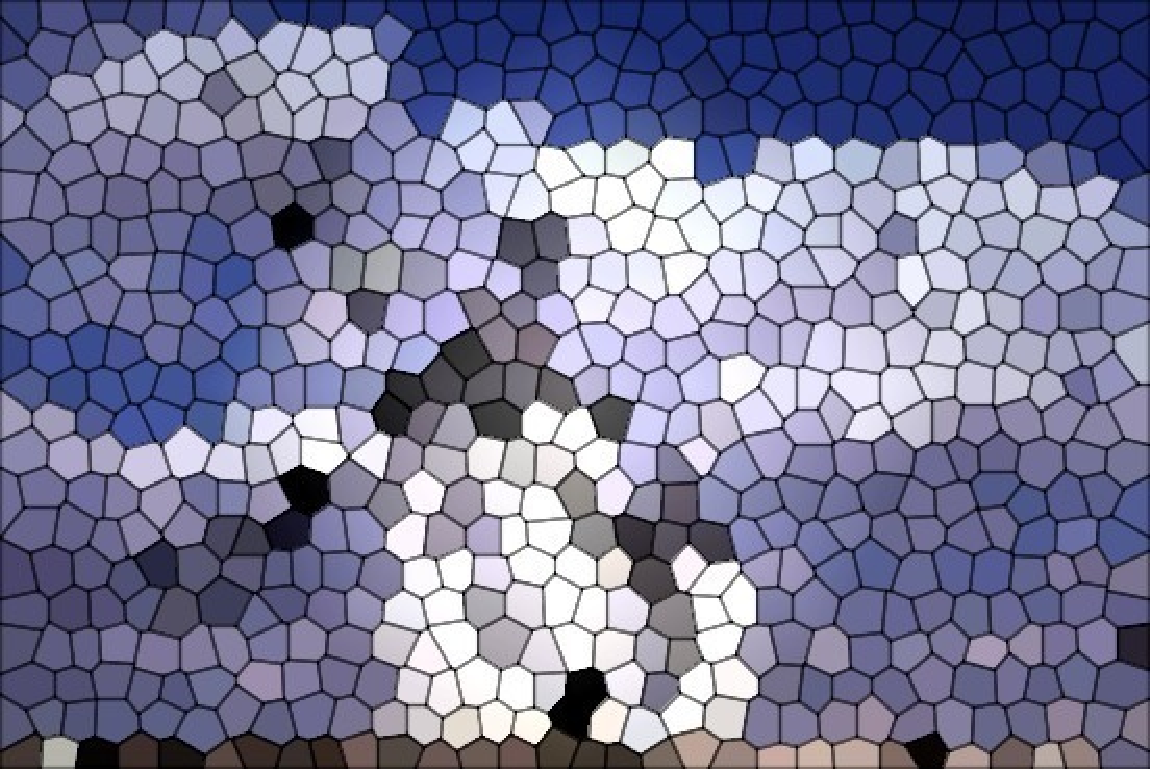
\includegraphics[scale=0.45]{img/introduccion/muestra_molino1}

\emph{¡Con una muestra pequeña es difícil averiguar el contenido de la imagen!}
\end{center}
\end{frame}
\note{Para entender a qué nos referimos cuando hablamos de un tamaño muestral suficiente para comprender lo que ocurre
en la población, podemos utilizar el siguiente símil en que se trata de comprender el motivo que representa una
fotografía.

Como sabéis, una fotografía digital está formada por multitud de pequeños puntitos llamados píxeles que se dispone
en una enorme tabla de filas y columnas (cuantas más filas y columnas haya se habla de que la foto tiene más
resolución). Aquí la población estaría formada por todos y cada uno de los píxeles que forman la foto. Por otro lado cada
pixel tiene un color y es la variedad de colores a lo largo de los pixels la que permite formar la imagen de la
fotografía.

Supongamos que queremos comprender el motivo de la fotografía y para ello tomamos sólo una pequeña muestra de los píxeles
de ella, como esta que aparece en la pantalla. ¿Serías capaz de averiguar de qué se trata?

Seguramente no has podido averiguar el motivo de la fotografía, porque en este caso el número de píxeles que hemos tomado
en la muestra es insuficiente para comprender toda la variabilidad de colores que hay en la foto.
}


%---------------------------------------------------------------------slide----
\begin{frame}
\frametitle{Determinación del tamaño muestral}
\framesubtitle{Muestra mayor de los píxeles de una imagen}
\mode<article>{Seguramente no has podido averiguar el motivo de la fotografía, porque en este caso el número de píxeles que hemos tomado en la muestra es insuficiente para comprender toda la variabilidad de colores que hay en la foto.

La siguiente imagen contiene una muestra mayor de píxeles.}
\begin{center}
¿Eres capaz de adivinar el motivo de la foto ahora?


\includegraphics[scale=0.45]{img/introduccion/muestra_molino2}

\emph{¡Con una muestra mayor es más fácil averiguar el contenido de la imagen!}
\end{center}
\end{frame}
\note{Sin embargo, si tomamos una muestra mayor, como esta otra, seguramente que ya si sabrías decir cuál es la imagen
de la foto. ¿Eres capaz?
}


%---------------------------------------------------------------------slide----
\begin{frame}
\frametitle{Determinación del tamaño muestral}
\framesubtitle{Población completa de los píxeles de una imagen}
\begin{center}
Y aquí está la población completa

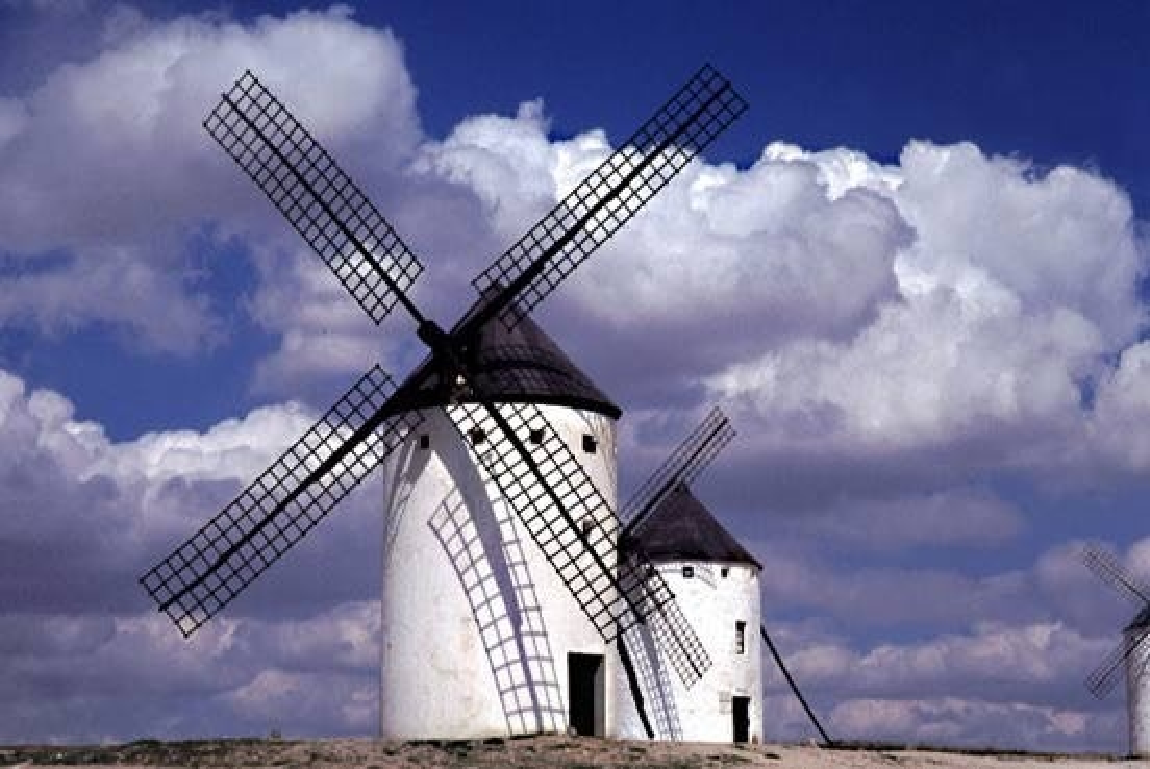
\includegraphics[scale=0.45]{img/introduccion/muestra_molino3}

\emph{¡No es necesario conocer todos los píxeles para averiguar la imagen!}
\end{center}
\end{frame}
\note{
Efectivamente, se trata de unos molinos de viento, y si has sido capaz de averiguarlo es porque en la segunda muestra el número de píxeles tomados en la muestra era suficiente para comprender el motivo de la fotografía.

Evidentemente, cuanto mayor sea la variabilidad de colores de la fotografía, mayor será el tamaño muestral requerido
para comprender el motivo de la foto, y cuanto menos variabilidad de colores haya en la foto, menos pixels habrá que
tomar, hasta el punto de que en una foto donde no hubiese variabilidad de colores, es decir, donde todos los pixels
tuviesen el mismo color, bastaría con tomar un pixel para conocer el motivo de la foto.

Bien, pues esto mismo pasa en las poblaciones que estudiaremos en el ámbito de las Ciencias de la Salud.
}

%---------------------------------------------------------------------slide----
\begin{frame}
\frametitle{Tipos de razonamiento}

\begin{center}
\tikzsetnextfilename{introduccion/tipos_razonamiento}
\resizebox{0.5\textwidth}{!}{% Autor: Alfredo Sánchez Alberca (email:asalber@ceu.es)
\begin{tikzpicture}[every label/.style={text=color1}]
\tikzstyle{node} = [align=center, node distance=1cm]; 
\tikzstyle{arrow} = [-latex, color1, line width=10pt];

\node (population) [label=90:Población] at (0,5) {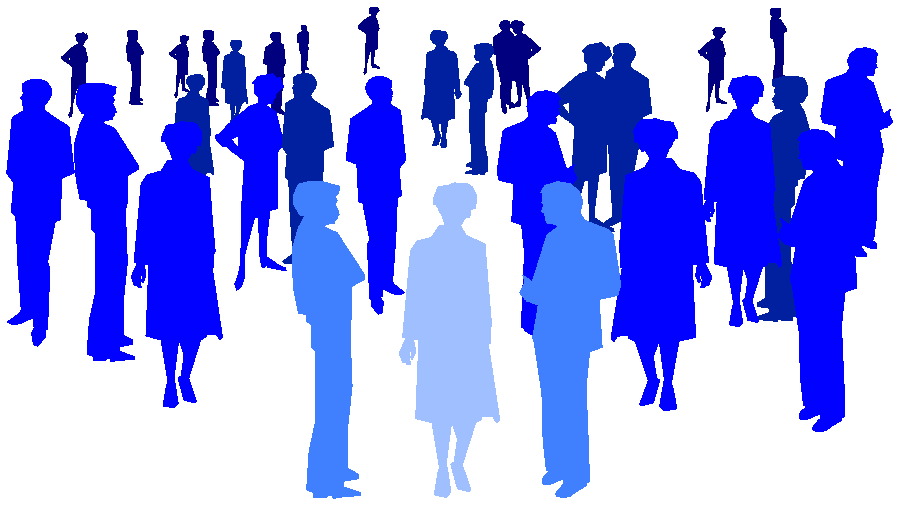
\includegraphics[height=2cm]{img/introduccion/poblacion.pdf}}; 
\node (sample) [label=-90:Muestra] at (0,0) {
\includegraphics[height=2cm]{img/introduccion/muestra.png}};
\node at (-0.5,2.6) [fill=color1,single arrow,shape border rotate=270,text=white, minimum width=1.2cm]{
\rotatebox{90}{Deducción}\phantom{}};
\node[node] at (-2,2.5) {De lo general\\ a lo particular};
\pause
\node at (0.5,2.4) [fill=color1,single arrow,shape border rotate=90,text=white, minimum width=1.2cm]{
\rotatebox{-90}{Inducción}\phantom{}};
\node[node] at (2.1,2.5) {De lo particular\\ a lo general};
\end{tikzpicture} }
\end{center}
\end{frame}
\note{Como se ha dicho antes, habitualmente realizaremos el estudio de la población a partir de muestras y luego
trataremos de extrapolar lo observado en la muestra al resto de la población. A este tipo de razonamiento que saca
conclusiones desde la muestra hacia la población se le conoce como razonamiento inductivo.

A diferencia del razonamiento deductivo que va de lo general a lo particular, o en nuestro caso de la población a la
muestra, el razonamiento inductivo no garantiza la certeza de las conclusiones, por lo que debemos ser cuidadosos a la
hora de generalizar sobre la población lo observado en al muestra, ya que si no se hacen bien las cosas podrían
cometerse errores.

Seguramente muchos habréis oído hablar de aquel científico loco que no sabía porqué la gente se emborrachaba y decidió
experimentar. Un día probó whisky con leche, y se emborrachó, otro día probó ron con leche y se emborrachó, y otro día
probó ginebra con leche y también se emborrachó. ¿Sabéis cuál es la conclusión a la que llegó? Efectivamente, concluyó
en su estudio que la causa de la embriaguez era la leche.

En este caso, el científico loco aplicó bien el método inductivo, sin embargo, las conclusiones fueron falsas porque no
hico un buen diseño del experimento y porque la muestra de bebidas tomadas no era representativa. Si hubiese mezclado la
leche con agua, habría visto enseguida que la leche no era la causa de su embriaguez.

Esto mismo podría ocurrir en nuestros estudios, si no tenemos cuidado a la hora de diseñar el experimento, y sobre todo,
si no tomamos una muestra representativa de la población. Cuando hablamos de que una muestra sea representativa, nos
referimos a que refleje las mismas características de la población de la que se ha tomado, pero a pequeña escala. Más
adelante veremos cómo debemos tomar la muestra para garantizar su representatividad.
}


%---------------------------------------------------------------------slide----
\begin{frame}
\frametitle{Tipos de razonamiento}
\begin{description}
\item [Características de la deducción:] Si las premisas son ciertas, garantiza la certeza de las conclusiones (es decir, si algo se cumple en la población, también se cumple en la muestra). Sin embargo, \alert{\emph{¡no aporta conocimiento nuevo!}}
\item [Características de la inducción:] No garantiza la certeza de las conclusiones (si algo se cumple en la muestra, puede que no se cumpla en la población, así que ¡cuidado con las extrapolaciones!).
Sin embargo, \alert{\emph{¡es la única forma de generar conocimiento nuevo!}}
\end{description}

La estadística se apoya fundamentalmente en el razonamiento inductivo ya que utiliza la información obtenida a partir de muestras para sacar conclusiones sobre las poblaciones.
\end{frame}


\subsection{Muestreo}
%---------------------------------------------------------------------slide----
\begin{frame}
\frametitle{Muestreo}
\begin{definicion}[Muestreo]
El proceso de selección de los elementos que compondrán una muestra se conoce como \emph{muestreo}.
\end{definicion}
\begin{center}
\tikzsetnextfilename{introduccion/muestreo}
\resizebox{0.8\textwidth}{!}{% Autor: Alfredo Sánchez Alberca (email:asalber@ceu.es)
\begin{tikzpicture}[every label/.style={text=color1}]
\tikzstyle{node} = [align=center, node distance=1cm]; 
\tikzstyle{arrow} = [-latex, color1, line width=12pt];

\node (population) [label=-90:Población] at (0,0) {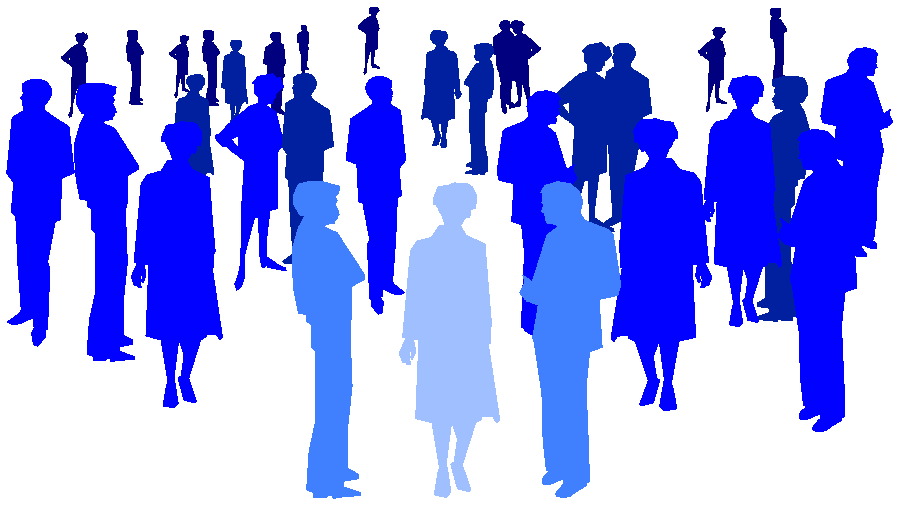
\includegraphics[height=2cm]{img/introduccion/poblacion.pdf}}; 
\node (sample) [label=-90:Muestra] at (6,0) {
\includegraphics[height=2cm]{img/introduccion/muestra.png}};
\node at (3.3,0) [fill=color1,single arrow,shape border rotate=0,text=white, minimum width=1.2cm]{
\ Muestreo\ \phantom{}};
\end{tikzpicture} }
\end{center}
Para que una muestra refleje información fidedigna sobre la población global debe ser representativa de la misma, lo que significa que debe reproducir a pequeña escala la variabilidad de la población.

\begin{center}
\alert{\emph{El objetivo es obtener una muestra representativa de la población.}}
\end{center}
\end{frame}
\note{En Estadística, al proceso por el cual se seleccionan a los individuos de la muestra se le llama muestreo.

Y como hemos visto antes, es muy importante que la muestra sea representativa de la población para que podamos sacar
conclusiones fiables sobre la población.
}


%---------------------------------------------------------------------slide----
\begin{frame}
\frametitle{Modalidades de muestreo}
Existen muchas técnicas de muestreo pero se pueden agrupar en dos categorías:
\begin{description}
\item[Muestreo Aleatorio] Elección aleatoria de los individuos de la muestra.
Todos tienen la misma probabilidad de ser elegidos (\emph{equiprobabilidad}).
\item[Muestreo No Aleatorio:] Los individuos se eligen de forma no aleatoria.
Algunos individuos tienen más probabilidad de ser seleccionados que otros.
\end{description}
Sólo las técnicas aleatorias evitan el sesgo de selección, y por tanto,  garantizan la representatividad de la muestra extraída, y en consecuencia la validez de las conclusiones.

Las técnicas no aleatorias no sirven para hacer generalizaciones, ya que no garantizan la representatividad de la muestra.
Sin embargo, son menos costosas y pueden utilizarse en estudios exploratorios.
\end{frame}
\note{En general, existen puchos procedimientos para seleccionar a los individuos de la muestra, pero se suelen dividir
en dos tipos:
\begin{description}
\item[Muestreo Aleatorio] Que se caracteriza por la elección aleatoria de los individuos de la muestra. Es decir los
individuos se eligen al azar, lo cual quiere decir que todos los individuos de la población tienen la misma probabilidad
de ser elegidos en la muestra.
\item[Muestreo No Aleatorio:] Que es cuando los individuos se eligen de forma no aleatoria.
\end{description}

Bien, debemos tener presente que sólo las técnicas aleatorias evitan el sesgo de selección, y por tanto, garantizan
la representatividad de la muestra extraída, y en consecuencia la validez de la inferencia que hagamos sobre la
población. Por tanto siempre que queramos sacar conclusiones fiables sobre la población debemos utilizar muestreos
aleatorios.

Las técnicas no aleatorias no sirven para hacer generalizaciones, ya que no garantizan la representatividad de la muestra.
Sin embargo, son menos costosas y pueden utilizarse en estudios exploratorios. En muchos estudios no tendremos
capacidad para hacer una elección aleatoria de los individudos de la muestra y nos tendremos que conformar con una
muestra dada. En estos casos no deberíamos hacer generalizaciones sobre la población y deberíamos ser muy cautelosos a
la hora de sacar conclusiones sobre esta.
}


%---------------------------------------------------------------------slide----
\begin{frame}
\frametitle{Muestreo aleatorio simple}
Dentro de las modalidades de muestreo aleatorio, el tipo más conocido es el \emph{muestreo aleatorio simple}, caracterizado por:
\begin{itemize}
\item Todos los individuos de la población tienen la misma probabilidad de ser elegidos para la muestra.
\item La selección de individuos es con reemplazamiento, es decir, cada individuo seleccionado es devuelto a la población antes de seleccionar al siguiente (y por tanto no se altera la población de partida).
\item Las sucesivas selecciones de un individuo son independientes.
\end{itemize}
La única forma de realizar un muestreo aleatorio es asignar un número a cada individuo de la población (\emph{censo}) y realizar un sorteo aleatorio.
\end{frame}
\note{La técnica de muestreo aleatorio más conocida es el muestreo aleatorio simple, que se caracteriza por tres
propiedades:
\begin{itemize}
\item Todos los individuos de la población tienen la misma probabilidad de ser elegidos para la muestra. Si no no sería
aleatorio.
\item La selección de individuos es con reemplazamiento, es decir, tras seleccionar a un individuo se devuelve a la
población antes de realizar la siguiente elección. Esto tiene el riesgo de incluir al mismo individuo varias veces en
la muestra, aunque en la práctica, con poblacione grandes es casi imposible, pero a cambio se consigue que no se altere
la población de partida.
\item Las sucesivas selecciones de un individuo son independientes, y por tanto la elección de un determinado individuo
no influye en la elección o no de otros.
\end{itemize}

En general, existen bastantes dudas en la comunidad científica sobre lo que es un muestreo aleatorio y lo que no lo es.
Por ejemplo, mucha gente piensa que hacer una encuesta a pie de calle es un muestreo aleatorio, pero en realidad no lo
es porque no todas las personas de la población tienen las misma probabilidad de ser encuestadas (hay gente que ni
siquiera sale a la calle). La única manera de garantizar que un muestreo es aleatorio es disponiendo de un censo de la
población de manera que todos y cada uno de los individuos tengan un número identificativo único y realizando un sorteo,
como el de la lotería, para extraer los identificadores de los individuos que formarán parte de la muestra. Este sorteo
se suele hacer habitualmente mediante algún programa informático que genere números de forma aleatoria.
}


\subsection{Variables estadísticas}

%---------------------------------------------------------------------slide----
\begin{frame}
\frametitle{Variables estadísticas y datos}
Todo estudio estadístico comienza por la identificación de las características que interesa estudiar en la población y que se medirán en los individuos de la muestra.
\begin{definition}[Variable estadística]
Una \emph{variable estadística} es una propiedad o característica medida en los individuos de la población.

Los \emph{datos} son los valores observados en las variables estadísticas.
\end{definition}

\begin{center}
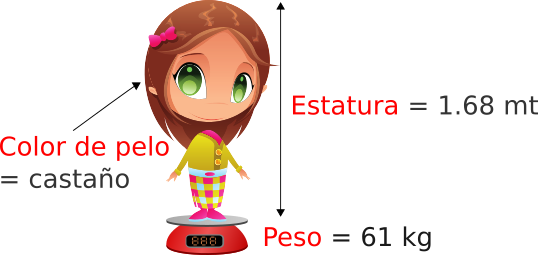
\includegraphics[scale=0.5]{img/introduccion/variables_estadisticas.png}
\end{center}
\end{frame}


%---------------------------------------------------------------------slide----
\begin{frame}
\frametitle{Variables estadísticas y atributos}
De acuerdo a la naturaleza de los valores y su escala, se tiene:
\begin{itemize}
\item \highlight{Variables cualitativas o atributos:} Miden cualidades no numéricas.
Pueden ser:
\begin{itemize}
\item \highlight{Nominales:} No existe un orden natural entre las categorías.\\
Ejemplo: El color de pelo o el sexo.
\item \highlight{Ordinales:} Existe un orden natural entre las categorías.\\
Ejemplo: El nivel de estudios o la gravedad de una enfermedad.
\end{itemize}
\item \highlight{Variables cuantitativas:} Miden cantidades numéricas.
Pueden ser:
\begin{itemize}
\item \highlight{Discretas:} Toman valores numéricos aislados (habitualmente números enteros).\\
Ejemplo: El número de hijos o de coches en una familia.
\item \highlight{Continuas:} Pueden tomar cualquier valor en un intervalo real.\\
Ejemplo: La estatura, el peso, o la edad de una persona.
\end{itemize}
\end{itemize}
\note{Todo estudio estadístico comienza por la identificación de las características que interesa estudiar en la
población y que se medirán en los individuos de la muestra. Estas características pueden ser de dos tipos según sean de
naturaleza cuantitativa o cualitativa, es decir, si miden cantidades o cualidades. Las características de naturaleza
cualitativa se conocen como atributos o variables cualitativas, mientras que las de naturaleza cuantitativas se conocen
como variables estadísticas o cuantitativas.

Los atributos, a su vez, pueden ser de dos tipos, nominales, cuando no existe un orden natural entre las modalidades o
valores que puede tomar el atributo, como por ejemplo el color de ojos, que puede ser negro, azul, verde, etc. pero no
tiene sentido ordenar los colores; u ordinales, cuando existe un orden natural entre las modalidades, como por ejemplo
el grado de gravedad de un paciente que puede ir de leve, moderado, grave o muy grave siguiendo un orden de menor a
mayor gravedad.

Por su parte las variables estadísticas también pueden clasificarse como discretas, cuando toman valores aislados que
suelen ser números enteros, como por ejemplo el número de hijos de una familia, que puede ser 0, 1, 2, 3, es decir, un
número entero posito pero no puede tomar valores decimales como 1.27; o continuas cuando si pueden tomar cualquier
valor dentro de un intervalo real, como por ejemplo la estatura, donde, entre dos estaturas cualesquiera como 1.60 y
1.70 podemos encontrar infinitas estaturas posibles.

Conocer el tipo de las variables u atributos es fundamental pues las técnicas que se utilizarán
para describirlas dependen del tipo de característica.

A la hora de seleccionar las variables que se estudiarán conviene tomar todas las variables que puedan tener relación
con el fenómeno que se pretende estudiar, y en esto cabe más pecar por exceso que por defecto, ya que si con el
trascurso del estudio se observa que una variable no aporta nada, siempre se puede descartar a posteriori, mientras que
si se observa que falta una variable importante, en la mayoría de los casos no se podrá volver atrás para
medirla.

En el caso de las variables numéricas, es importante también explicitar las unidades en que van a medirse.
}
\end{frame}

%---------------------------------------------------------------------slide----
\begin{frame}
\frametitle{Tipos de variables estadísticas}
\begin{center}
\tikzsetnextfilename{introduccion/tipos_variables}
\resizebox{\textwidth}{!}{% Author: Alfredo Sánchez Alberca (email:asalber@ceu.es)
% Types of statistical variables
\tikzset{every node/.style = {align=center, inner sep=2pt, text centered}}
\begin{tikzpicture}[-, >=stealth', level distance = 1.5cm,
	level 1/.style={sibling distance = 6cm},
	level 2/.style={sibling distance = 3cm},
	level 3/.style={font=\small}
] 

\node [rectangle, minimum height=2cm, minimum width=\textwidth, fill=color2!30, rounded corners, opacity=0.5] at
(0,-4.5) {\phantom{0}}; 

\node {Variables estadísticas}
	child{node{Qualitativas}
		child{node{Nominales}
			child{node{Color de pelo\\ Sexo\\ Estado civil\\ $\vdots$}}
		}     
       	child{node{Ordinales}
			child{node{Nivel de estudios\\ Calificación\\ Talla de ropa\\ $\vdots$}}
		}           
    }
	child{node{Cuantitativas}
		child{node{Discretas}
			child{node{Número de hijos\\ Número de coches\\ Número de asignaturas\\ $\vdots$}}
		}     
        child{node{Continuas}
			child{node{Estatura\\ Peso\\ Edad\\ $\vdots$}}
%           	child{node{\parbox[top][1cm][t]{2cm}{Interval}}}
%            child{node{\parbox[top][1cm][t]{2cm}{Ratio}}}
        }               
    }
; 

\node [text=color1] at (0,-5.3) {Ejemplos};
\end{tikzpicture}}
\end{center}
\end{frame}



%---------------------------------------------------------------------slide----
\begin{frame}
\frametitle{Tipos de variables estadísticas}
\framesubtitle{Eligiendo la variable adecuada}
En ocasiones una característica puede medirse mediante variables de distinto tipo.

\textbf{Ejemplo} Si una persona fuma o no podría medirse de diferentes formas:
\begin{itemize}
\item Fuma: si/no. (Nominal)
\item Nivel de fumador: No fuma / ocasional / moderado / bastante / empedernido. (Ordinal)
\item Número de cigarros diarios: 0,1,2,\ldots (Discreta)
\end{itemize}

En estos casos es preferible usar variables cuantitativas a cualitativas.
Dentro de las cuantitativas es preferible usar las continuas a las discretas y dentro de las cualitativas es preferible usar ordinales a nominales pues aportan más información.

\begin{center}
\tikzsetnextfilename{introduccion/informacion_variables}
\scalebox{1}{% Author: Alfredo Sánchez Alberca (email:asalber@ceu.es)
% Plot with the level of information of each variable type
\begin{tikzpicture}[scale=0.5]
\tikzstyle{node} = [align=center, text=color1];
\useasboundingbox (-0.5,-0.5) rectangle (18.5,2.7);
\draw[stealth-stealth, thin, color1!90, line width=12pt] (-0.5,1.5) -- (18.5,1.5);
\node at (1.5,1.5) {\color{white}-- Info};
\node at (16.5,1.5) {\color{white} + Info};
\node[node] at (1,0) {Nominales};
\node[node] at (5,0) {Ordinales};
\node[node] at (9,0) {Discretas};
\node[node] at (13,0) {Intervalo};
\node[node] at (17,0) {Ratio};
\end{tikzpicture}}
\end{center}
\end{frame}


%---------------------------------------------------------------------slide----
\begin{frame}
\frametitle{Tipos de variables estadísticas}
De acuerdo al papel que juegan en el estudio:
\begin{itemize}
\item \highlight{Variables independientes:} Variables que supuestamente no dependen de otras variables en el estudio.
Habitualmente son las variables manipuladas en el experimento para ver su efecto en las variables dependientes.
Se conocen también como \emph{variables predictivas}.
\item \highlight{Variables dependientes:} Variables que supuestamente dependen de otras variables en el estudio.
No son manipuladas en el experimento y también se conocen como \emph{variables respuesta}.
\end{itemize}

\textbf{Ejemplo} En un estudio sobre el rendimiento de los alumnos de un curso, la inteligencia de los alumnos y el número de horas de estudio diarias serían variables independientes y la nota del curso sería una variable dependiente.
\end{frame}


%---------------------------------------------------------------------slide----
\begin{frame}
\frametitle{Tipos de estudios estadísticos}
\begin{itemize}
\item \highlight{Experimentales:} Cuando las variables independientes son manipuladas para ver el efecto que producen en las variables dependientes.\newline
\textbf{Ejemplo} En un estudio sobre el rendimiento de los estudiantes en un test, el profesor manipula la metodología de estudio para crear dos o más grupos con metodologías de estudio distintas.
\item \highlight{No experimentales:} Cuando las variables independientes no son manipuladas.
Esto no significa que sea imposible hacerlo, sino que es difícil o poco ético hacerlo.\newline
\textbf{Ejemplo} En un estudio un investigador puede estar interesado en el efecto de fumar sobre el cáncer de pulmón.
Aunque es posible, no sería ético pedirle a los pacientes que fumasen para ver el efecto que tiene sobre sus pulmones.
En este caso, el investigador podría estudiar dos grupos de pacientes, uno con cáncer de pulmón y otro sin cáncer, y observar en cada grupo cuántos fuman o no.
\end{itemize}

Los estudios experimentales permiten identificar causas y efectos entre las variables del estudio, mientras que los no experimentales sólo permiten identificar relaciones de asociación entre las variables.
\end{frame}


%---------------------------------------------------------------------slide----
\begin{frame}
\frametitle{La tabla de datos}
Las variables a estudiar se medirán en cada uno de los individuos de la muestra, obteniendo un conjunto de datos que suele organizarse en forma de matriz que se conoce como \structure{\textbf{tabla de datos}}.

En esta tabla cada columna contiene la información de una variable y cada fila la información de un individuo.

\textbf{Ejemplo}
\begin{center}
\begin{tabular}{|l|c|c|c|c|}
\hline
Nombre & Edad & Sexo & Peso (Kg) & Altura (cm)\\
\hline
José Luis Martínez & 18 & H &  85 & 179 \\
Rosa Díaz & 32 & M & 65 & 173 \\
Javier García & 24 & H & 71 & 181 \\
Carmen López & 35 & M &  65 & 170 \\
Marisa López  & 46 & M &  51 & 158 \\
Antonio Ruiz & 68 & H & 66 & 174 \\
\hline
\end{tabular}
\end{center}
\note{Una vez seleccionadas las variables, estas se medirán en cada uno de los invidividuos de la muestra con lo que se
obtendrá un conjunto de datos que se organiza en forma de matriz conocida como matriz de datos. Es importante organizar
la matriz de manera que en cada columna contenga la información de una variable y cada fila la información de un
individuo.

En este ejemplo puede observarse la matriz de datos correspondiente a una muestra de cinco individuos en los que se han
medido 4 características, tres variables, que son la Edad, el Peso y la Altura, y un atributo que es el Sexo. Como puede
apreciarse la primera columna contiene las edades de todos los individuos de la muestra, la segunda el sexo, la tercera
los pesos y la última las alturas, mientras la información de cada fila hace referencia al mismo individuo, de manera
que la primera fila, por ejemplo, contiene los datos de José Luis Martínez que tiene 18 años, es hombre, pesa 85 Kg y
mide 179 cm.
}
\end{frame}


\subsection{Fases del análisis estadístico}

%---------------------------------------------------------------------slide----
\begin{frame}
\frametitle{Fases del análisis estadístico}
Normalmente un estudio estadístico pasa por las siguientes etapas:
\begin{enumerate}
\item El estudio comienza por el diseño previo del mismo en el que se establezcan los objetivos del mismo, la población, las variables que se medirán y el tamaño muestral requerido.
\item A continuación se seleccionará una muestra representativa del tamaño establecido y se medirán las variables en los individuos de la muestra obteniendo la tabla de datos.
De esto se encarga el \textbf{Muestreo}.
\item El siguiente paso consiste en describir y resumir la información que contiene la muestra.
De esto se encarga la \textbf{Estadística Descriptiva}.
\item La información obtenida es proyectada sobre un modelo matemático que intenta explicar el comportamiento de la población y el modelo se valida.
De todo esto se encarga la \textbf{Estadística Inferencial}.
\item Finalmente, el modelo validado nos permite hacer predicciones y sacar conclusiones sobre la población de partida con cierta confianza.
\end{enumerate}
\end{frame}



%---------------------------------------------------------------------slide----
\begin{frame}
\frametitle{El ciclo estadístico}
\begin{center}
\tikzsetnextfilename{introduccion/ciclo_estadistico}
\resizebox{0.85\textwidth}{!}{% Author: Alfredo Sánchez Alberca (email:asalber@ceu.es)
% Plot with the phases of the statistical cycle
\begin{tikzpicture}[every label/.style={text=color1}]
\tikzstyle{arrow} = [-latex, color1, line width=12pt];
\tikzstyle{node} = [align=center, inner sep=10pt];
\node[node, label=-90:Población] (population) at (1,1)
{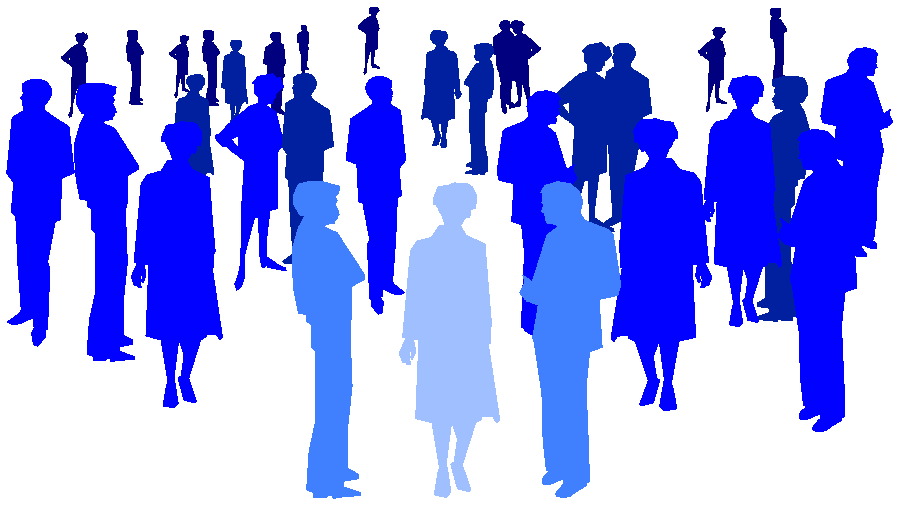
\includegraphics[height=1.5cm]{img/introduccion/poblacion}}; 
\pause
\node[node,label=90:Muestra] (sample) at
(1,6){
\includegraphics[height=1.5cm]{img/introduccion/muestra.png}}; 
\node at (1,3.4) [fill=color1,single arrow,shape border rotate=90,text=white, minimum width=1.2cm, minimum
height=3cm]{
\rotatebox{90}{Muestreo}\phantom{}};
\pause
\node[node,label=90:Resumen estadístico] (statistics) at (8,6) {\Large $\bar x$ \quad $s^2$\\\Large \quad $p$ \quad
$g_1$}; 
\node at (4.5,6) [fill=color1,single arrow,shape border rotate=0,text=white, minimum width=1.2cm, minimum
height=3cm]{
Estadística Descriptiva\phantom{}};
\pause
\node[node,label=-90:Modelo] (model) at (8,1) {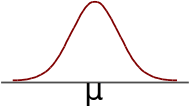
\includegraphics[scale=0.5]{img/introduccion/normal}};
\node at (8,3.6) [fill=color1,single arrow,shape border rotate=270,text=white, minimum width=1.2cm, minimum
height=3cm]{
\rotatebox{90}{Est. Inferencial}\phantom{}};
\pause
\node at (4.5,1) [fill=color1,single arrow,shape border rotate=180,text=white, minimum width=1.2cm, minimum
height=3cm]{ Predicción\phantom{}};
\end{tikzpicture}}
\end{center}
\end{frame}
\note{Para acabar con esta introducción a la Estadística, veremos cuáles son las fases por las que suele pasar cualquier
estudio estadístico, y las partes de la Estadística que se encargan de ello.

\begin{enumerate}
\item En general siempre partiremos de una población en la que queremos estudiar un fenómeno, y se hará un diseño previo del
estudio donde se formulen los objetivos del mismo, qué variables se medirán en los individuos de la población, qué
precisión queremos para nuestras conclusiones y qué tamaño muestral será necesario para ello.
\item A continuación se debe extraer una muestra representativa de la población y de esto esto se
encarga el \textbf{muestreo}.
\item El siguiente paso consiste en estudiar las muestra extraída y presentar de manera ordenada y resumida la
información que esta contiene. De esto se encarga la \textbf{estadística descriptiva}.
\item A continuación, la información obtenida es proyectada sobre un modelo matemático que intenta reflejar el
comportamiento de las variables estudiadas en la población. Tras construir este modelo, se deber realizar un
constraste o una crítica del mismo. Si lo que predice el modelo discrepa con lo observado en la muestra, habrá que
reformular el modelo o construir otro nuevo, mientras que si encaja en lo observado en la muestra, lo daremos por válido
y ello nos permitirá hacer predicciones sobre la población de partida con cierta fibilidad.
\end{enumerate}

En esta primera parte del curso nos centraremos en la Estadística Descriptiva, es decir, la que se encarga de describir
la información contenida en la muestra, pero debemos tener presente que la verdadera potencia de la Estadística está en
completar este ciclo y poder llegar a comprender y controlar el fenómeno que afecta a toda la población.
}
